
\chapter{Image file formats and steganography techniques}

\section{Introduction}

\setlength\columnsep{20pt}
\begin{multicols*}{2}
An image is a two-dimensional representation depicting any possible subject conceivable by human imagination, captured using an optical device (such as a camera or a telescope) or a natural object (human eyes). The image can then be rendered and displayed for other people to see either manually (by painting, carving etc.) or automatically (by using a computer). In this chapter we will focus on images captured using digital optical devices that are rendered automatically. The correct term for them is digital images, but throughout the rest of the paper they will be reffered to as images for convenience.

\begin{figure}[H]
    \centering
    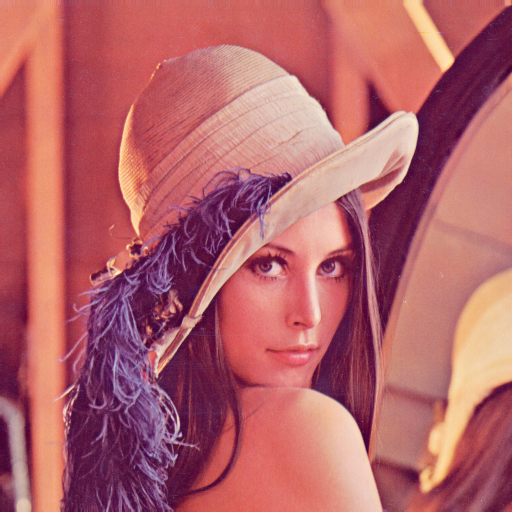
\includegraphics[width=5cm,height=5cm,keepaspectratio]{pics/lenna}
    \caption{Lenna - Classic example of digital image}
    \label{Lenna}
\end{figure}

Computers are programmed to do operations in a clear sequential way and this rule doesn't change when working with pictures. In order for a computer to be able to render an image, it needs to know some general metadata information about the photo, such as the width and height, as well as the data bytes of the image. These bytes are the actual representation of the picture which compose the two-dimensional pixel map\footnote{This is true for a lossless format, where each pixel is stored in memory. It is not exactly the case for lossy formats such as JPEG where the image goes through processing before being rendered. More information later in the chapter.}. A pixel is the smallest unit that a computer monitor can read and display. The pixel color is the result of merging the different color channels which compose the picture (such as RGB, YUV, YCbCr etc.). Here is an example of the entire process - let's assume that from the image data bytes the first 3 bytes have the decimal values 20, 127, 250 and that it uses the RGB color model. This means that when the computer will have to render the image, the first pixel will have the red component equal to 20 (0x14), the green equal to 127 (0x7F), and the blue equal to 250 (0xFA), in what will finally be interpreted as \#147FFA by the monitor (variation of light blue). 

\begin{figure}[H]
    \centering
    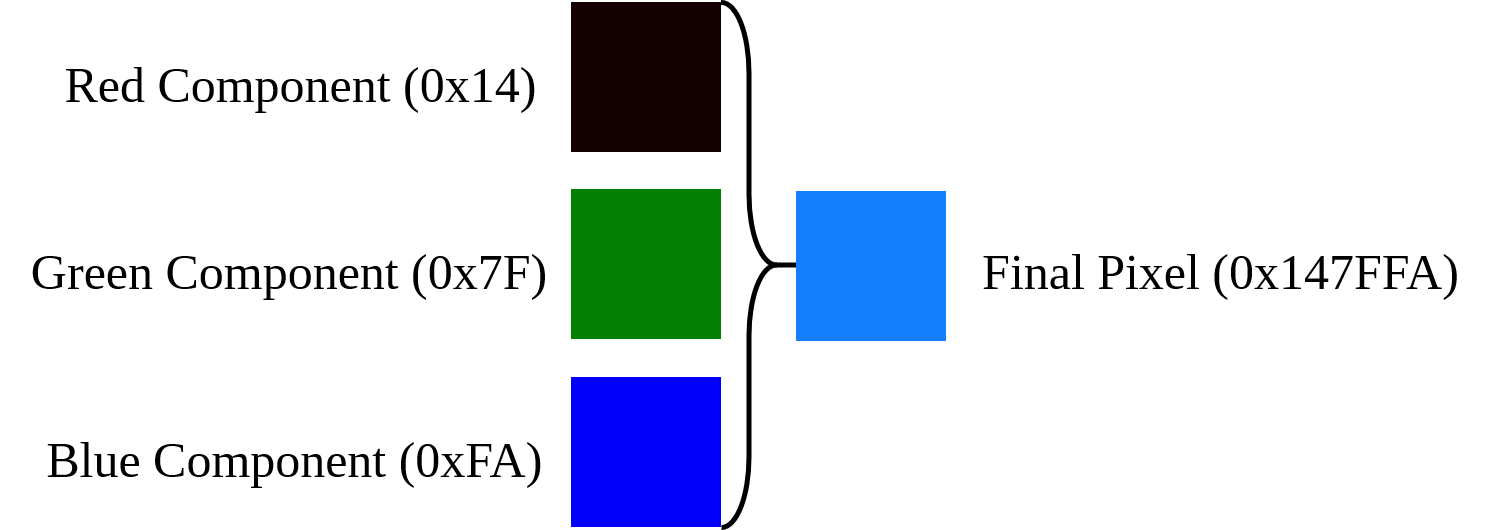
\includegraphics[width=8cm,height=2.7cm,keepaspectratio]{pics/how_a_pixel_works}
    \caption{How 3 colors channels build the pixel}
    \label{Pixel Creation}
\end{figure}

With all of this information in mind, we can now procede to discussing the different steganography methods possible when working with images as our cover.

\end{multicols*}


\section{General and particular algorithms in image steganography}
\subsection{Least Significant Bit (LSB)}
test1
\subsection{Metadata encoding}
test2
\subsection{Unused bytes}

\section{BitMap Picture (BMP)}

\section{Portable Network Graphics (PNG)}

\section{Joint Photographic Experts Group (JPEG)}